%% covariates.tex — Zurich Day 2 (afternoon): Covariates in DiD
%% Scott Cunningham, University of Zurich, May 12, 2026
%%
%% Compile: pdflatex covariates.tex
%% Style:   remix.sty (in same directory)
%%
%% Pedagogical structure: problem -> narrative -> picture -> codeblock -> intuition -> technical
%% Source material:
%%   /Users/scunning/Causal-Inference-2/Slides/Tex/02-Covariates.tex (heavy copy)
%%   /Users/scunning/the-remix-tour/zurich/decks/code/IPW-Demo/ (existing pscore-critique sim)
%%   /Users/scunning/Library/CloudStorage/.../readings/SantAnna_DiD_CompositionalChanges_text.md
%%
%% NEW pedagogical block: the "can't I just control for the pscore?" trap
%%   (Lesson 4). Built fresh from the IPW-Demo + zurich_content_map.md
%%   notes. Placed BEFORE DR so that DR's value is properly motivated.

\documentclass[aspectratio=169,11pt]{beamer}
\usepackage{remix}

\usepackage{tikz}
\usetikzlibrary{positioning,arrows.meta,calc,shapes.geometric,fit,backgrounds}
\usepackage{listings}
\usepackage{xcolor}
\usepackage{booktabs}
\usepackage{colortbl}

\lstset{
  basicstyle=\ttfamily\footnotesize,
  keywordstyle=\color{accentdark}\bfseries,
  commentstyle=\color{warmgray}\itshape,
  stringstyle=\color{ocean},
  backgroundcolor=\color{lightbg},
  frame=single,
  framesep=4pt,
  rulecolor=\color{warmgray!40},
  columns=fullflexible,
  showstringspaces=false,
  breaklines=true,
  numbers=none,
  xleftmargin=0.4em,
  xrightmargin=0.4em,
}

\renewcommand{\remixfooter}{University of Zurich\,\textperiodcentered\,Department of Economics\,\textperiodcentered\,May 2026}

\begin{document}

%% =====================================================================
%%                                ACT I
%% =====================================================================

%% ---------- Slide 1: TITLE ----------
\remixtitleframe
  {Covariates in DiD}
  {Day 2 of 3: Afternoon}
  {Scott Cunningham \textperiodcentered\ Baylor University}
  {University of Zurich \textperiodcentered\ May 12, 2026}

%% ---------- Slide 2: Where we are ----------
\begin{frame}{The PT-violation problem, take two}
\vspace{0.5em}
\begin{itemize}
  \item This morning: a \highlight{third group} that shares the differential trend.
  \item But often, you don't have a clean placebo group.
  \item This afternoon: \highlight{condition on covariates that absorb the differential trend.}
\end{itemize}
\vspace{0.6em}
\begin{block}{Today's three estimators, and one false friend}
\small
\textbf{OR} (outcome regression) \;\; \textbf{IPW} (inverse propensity weighting) \;\; \textbf{DR} (doubly robust) \\[0.3em]
And: ``\textit{can't I just control for the propensity score in a regression?}'' \\
\highlight{That's the false friend.} We'll see why before DR.
\end{block}
\end{frame}

%% ---------- Slide 3: The applied problem ----------
\begin{frame}{The applied problem}
\vspace{0.5em}
\begin{itemize}
  \item Your treated states differ from your controls on observables --- baseline income, demographics, industry mix, education.
  \item If $Y(0)$ trends differ across these dimensions, unconditional PT is implausible.
  \item But maybe \textit{within} strata of $X$, PT holds:
\end{itemize}
\vspace{0.4em}
\begin{center}
\small
$\mathbb{E}[\Delta Y(0) \mid D=1, X] \;=\; \mathbb{E}[\Delta Y(0) \mid D=0, X]$
\end{center}
\vspace{0.5em}
\begin{itemize}
  \item This is \highlight{conditional parallel trends}. The escape valve for designs without a placebo group.
  \item Three estimators target this. They differ in \textit{which side} of the conditioning they model.
\end{itemize}
\end{frame}

%% ---------- Slide 4: Today's seven beats ----------
\begin{frame}{This afternoon, seven beats}
\vspace{0.3em}
\begin{enumerate}\small
  \item Conditional parallel trends --- the identifying assumption we'll lean on
  \item OLS-with-controls: the bias decomposition that drives demand for everything below
  \item Outcome regression (Heckman-Ichimura-Todd)
  \item Inverse propensity weighting (Abadie 2005)
  \item \textit{The trap}: ``can't I just control for the propensity score?''
  \item Doubly robust DiD (Sant'Anna \& Zhao 2020)
  \item Hidden linearity bias --- TWFE-with-controls fully exposed (Caetano \& Callaway 2024)
\end{enumerate}
\vspace{0.4em}
\begin{center}
\small\color{warmgray}\itshape
We lead with the bias of OLS. \;\;Each fix below removes one piece of that bias.
\end{center}
\end{frame}

%% =====================================================================
%%                                LESSON 1
%% =====================================================================
\remixsection{1.\ Conditional Parallel Trends}

%% ---------- L1-F1: the assumption ----------
\begin{frame}{Conditional parallel trends, formally}
\vspace{0.4em}
\begin{block}{The new identifying assumption}
\small
\centering
$\mathbb{E}[\Delta Y(0) \mid D{=}1, X] \;=\; \mathbb{E}[\Delta Y(0) \mid D{=}0, X]$
\end{block}
\vspace{0.5em}
\begin{itemize}\small
  \item Within strata of $X$, the untreated trend is the same for treated and control.
  \item Equivalently: \textit{any} differential trend across treated and control is fully explained by their differences in $X$.
  \item Trade-off: weaker than unconditional PT (good), but you have to pick the right $X$ (hard).
  \item Two ways to use $X$: model the outcome side ($\mu(X)$), or model the treatment side ($p(X)$). Each is one of our estimators.
\end{itemize}
\end{frame}

%% ---------- L1-F2: picking covariates ----------
\begin{frame}{Picking $X$: pre-treatment confounders, not post-treatment outcomes}
\vspace{0.4em}
\begin{itemize}\small
  \item You want $X$ that (i) predicts the treatment (causes selection) AND (ii) predicts $Y(0)$ (causes outcome differences).
  \item \highlight{Pre-treatment} only. Post-treatment $X$ may be affected by $D$ and will leak.
  \item Three practical screens (Imbens-Rubin, normalized differences):
  \begin{itemize}\small
    \item[--] Drop treated post-period, regress $Y(0)$ on candidate $X$
    \item[--] Within control units, regress $Y(0)$ on candidate $X$
    \item[--] Use $t{-}2$ and $t{-}1$ to estimate $\Delta Y(0)$ and regress on $X$
  \end{itemize}
\end{itemize}
\vspace{0.3em}
\meta{Source: Imbens \& Rubin (2015); \texttt{02-Covariates.tex} frames 156--183.}
\end{frame}

%% =====================================================================
%%                                LESSON 2
%% =====================================================================
\remixsection{2.\ Outcome Regression \\[0.3em] {\normalsize\normalfont What OLS-with-controls gives you --- and what it doesn't}}

%% ---------- L2-F0a: Lead with the bias decomposition ----------
\begin{frame}{Before any fix: what does OLS-with-controls actually identify?}
\vspace{0.4em}
The workhorse: $Y_{it} = \alpha_i + \gamma_t + \alpha\, D_{it} + \theta\, X_{it} + \varepsilon_{it}$. Estimate $\widehat\alpha$ by TWFE-OLS.
\vspace{0.5em}
\begin{block}{The Caetano-Callaway (2024) decomposition}
\vspace{-0.2em}
\centering
$\widehat{\alpha}_{\text{TWFE+}X} \;\;\xrightarrow{p}\;\; \underbrace{\overline{\text{ATT}}_w}_{\text{weighted ATT}} \;\;+\;\; \mathrm{Bias}_A \;\;+\;\; \mathrm{Bias}_B \;\;+\;\; \mathrm{Bias}_C$
\end{block}
\vspace{0.5em}
\begin{itemize}\small
  \item It is \textit{not} the ATT.\;\; It is a \textit{weighted average} of conditional ATTs --- possibly with perverse weights --- \textbf{plus} three bias terms.
  \item Each bias is a different assumption silently being made.
  \item \highlight{The bias is what creates the demand for OR, IPW, and DR.} They are each fixes for a piece of this expression.
\end{itemize}
\end{frame}

%% ---------- L2-F0b: read the three bias terms ----------
\begin{frame}{The three bias terms, named}
\footnotesize
\begin{block}{Bias A: heterogeneous $\tau$ in $X$}
Treatment effect varies with $X$, but TWFE fits one $\theta$. \;\highlight{Proof: next 4 slides (steps 1--4).}
\end{block}
\begin{block}{Bias B: non-parallel $X$-trends across treated and control}
$Y^0$ trends depend on $X$ in different ways for treated vs.\ control. \;\highlight{Proof: 3 slides after that (steps 5--7).}
\end{block}
\begin{block}{Bias C: the FE transformation drops $X$-levels and time-invariant $Z$}
What you wrote as a control isn't what you ended up conditioning on. \;\highlight{Lesson 6.}
\end{block}
\begin{center}
\footnotesize\color{warmgray}\itshape
Three failures, three fixes. \;OR addresses A; IPW addresses A and B differently; DR closes both at once.
\end{center}
\end{frame}

%% ---------- L2-F1: OR narrative ----------
\begin{frame}{Outcome regression: model the trend, impute the counterfactual}
\vspace{0.5em}
\textbf{Heckman, Ichimura \& Todd (1997).}
\vspace{0.4em}
\begin{enumerate}
  \item Use \textit{only the control group} to fit a model of $\Delta Y$ on $X$:
  \begin{center}\small $\widehat{\mu}_0(X) \;=\; \widehat{\mathbb{E}}[\Delta Y \mid D{=}0, X]$ \end{center}
  \item For each treated unit, predict the counterfactual trend $\widehat{\mu}_0(X_i)$.
  \item The OR-DiD estimator:
  \begin{center}
  \small
  $\widehat{\delta}_{\text{OR}} \;=\; \dfrac{1}{N_1}\displaystyle\sum_{i:\, D_i=1}\big(\Delta Y_i \;-\; \widehat{\mu}_0(X_i)\big)$
  \end{center}
\end{enumerate}
\vspace{0.4em}
\highlight{Interpretation:} OR \textit{imputes} what the treated would have done if untreated --- using only the control group's $X$-to-trend mapping.
\end{frame}

%% ---------- L2-F2: TWFE with controls ----------
\begin{frame}{The TWFE-with-controls regression --- and the three assumptions it hides}
\vspace{0.4em}
\[
Y_{it} \;=\; \alpha_i \;+\; \gamma_t \;+\; \delta\, (T_t \times D_i) \;+\; \theta\, X_{it} \;+\; \varepsilon_{it}
\]
\vspace{0.1em}
\begin{itemize}\small
  \item Standard move: add $X_{it}$ to the TWFE. \;\; \textit{``Sure! If you're willing to impose three more assumptions.''}
  \item \textbf{(1) Additive functional form} in $X$ (linear, no $D \times X$ interaction).
  \item \textbf{(2) Homogeneous treatment effects} in $X$ (the slope $\theta$ doesn't depend on $D$).
  \item \textbf{(3) No $X$-specific trends differing across treated and control.}
\end{itemize}
\vspace{0.4em}
\begin{center}
\small\color{warmgray}\itshape
Next slide: the proof of (2). Where does the homogeneity-in-$X$ assumption come from? Trace it through the conditional expectations.
\end{center}
\end{frame}

%% ---------- L2-F2b: PROOF step 1 — TWFE-with-X and the conditional-PT identity ----------
\begin{frame}{Proof, step 1 --- the TWFE model and what conditional PT gives us}
\vspace{0.4em}
\textbf{The TWFE model with one covariate $X$:}
\[
Y_{it} \;=\; \alpha_1 + \alpha_2\, T_t + \alpha_3\, D_i + \delta\,(T_t \times D_i) + \theta\, X_{it} + \varepsilon_{it}.
\]
\vspace{0.3em}
\textbf{Conditional parallel trends} says, for each value of $X$:
\[
\mathbb{E}[Y^0_1 - Y^0_0 \mid D{=}1, X] \;=\; \mathbb{E}[Y^0_1 - Y^0_0 \mid D{=}0, X].
\]
\vspace{0.1em}
Rearrange. The missing counterfactual for the treated is identified:
\[
\mathbb{E}[Y^0_1 \mid D{=}1, X] \;=\; \mathbb{E}[Y_0 \mid D{=}1, X] + \mathbb{E}[Y_1 \mid D{=}0, X] - \mathbb{E}[Y_0 \mid D{=}0, X].
\]
\vspace{0.2em}
\begin{center}
\footnotesize\color{warmgray}\itshape
Three observed conditional means $\Rightarrow$ one unobserved counterfactual. \;That's all PT does for us.
\end{center}
\end{frame}

%% ---------- L2-F2c: PROOF step 2 — plug TWFE in, the slopes look the same ----------
\begin{frame}{Proof, step 2 --- plug TWFE in, the slopes look the same}
\vspace{0.4em}
\textbf{From the TWFE model, the observed conditional means are:}
\begin{align*}
\mathbb{E}[Y_0 \mid D{=}1, X] &= \alpha_1 + \alpha_3 + \theta\, X \\
\mathbb{E}[Y_1 \mid D{=}0, X] &= \alpha_1 + \alpha_2 + \theta\, X \\
\mathbb{E}[Y_0 \mid D{=}0, X] &= \alpha_1 + \theta\, X
\end{align*}
\textbf{Plug into the identity from step 1:}
\[
\mathbb{E}[Y^0_1 \mid D{=}1, X] \;=\; \alpha_1 + \alpha_2 + \alpha_3 + \theta\, X.
\]
\textbf{The treated $Y^1$ post-period, from the TWFE model:}
\[
\mathbb{E}[Y^1_1 \mid D{=}1, X] \;=\; \alpha_1 + \alpha_2 + \alpha_3 + \delta + \theta\, X.
\]
\begin{center}
\footnotesize\color{warmgray}\itshape
Both potential outcomes carry the \textit{same} $\theta$ in $X$. \;Subtract: ATT $= \delta$. \;Clean. \;\textit{Suspiciously clean.}
\end{center}
\end{frame}

%% ---------- L2-F2d: PROOF step 3 — what if the two slopes differ? ----------
\begin{frame}{Proof, step 3 --- what if $Y^1$ and $Y^0$ have different slopes in $X$?}
\vspace{0.4em}
\textbf{Let the slopes differ.} \;Write $\theta_1$ for the $Y^1$ slope and $\theta_2$ for the $Y^0$ slope:
\begin{align*}
\mathbb{E}[Y^1_1 \mid D{=}1, X] &= \alpha_1 + \alpha_2 + \alpha_3 + \delta + \boxed{\theta_1}\, X \\
\mathbb{E}[Y^0_1 \mid D{=}1, X] &= \alpha_1 + \alpha_2 + \alpha_3 \phantom{\;+\;\delta} + \boxed{\theta_2}\, X
\end{align*}
\vspace{0.1em}
\textbf{The true ATT given $X$:}
\[
\text{ATT}(X) \;=\; \mathbb{E}[Y^1 - Y^0 \mid D{=}1, X] \;=\; \delta \;+\; (\theta_1 - \theta_2)\, X.
\]
\vspace{0.2em}
\begin{itemize}\small
  \item If $\theta_1 \neq \theta_2$, the treatment effect \textit{depends on $X$}.
  \item TWFE fits \highlight{one} $\theta$, not two.
  \item So $\widehat{\delta}$ recovers the ATT only when $\theta_1 = \theta_2$.
\end{itemize}
\end{frame}

%% ---------- L2-F2e: PROOF step 4 — the named assumption ----------
\begin{frame}{Proof, step 4 --- the named assumption: \textit{homogeneous} $\tau$ in $X$}
\vspace{0.5em}
\begin{block}{Assumption}
\centering
\textbf{TWFE-with-$X$ requires the treatment effect to be the same at every value of $X$.}
\end{block}
\vspace{0.6em}
\begin{itemize}
  \item If $X$ is \textbf{sex}: the effect is the same for men and for women.
  \item If $X$ is \textbf{income} (continuous): the effect is the same at \$1 and at \$1{,}000{,}000.
  \item If $X$ is \textbf{age}: the effect is the same at 25 and at 65.
\end{itemize}
\vspace{0.6em}
\begin{center}
\small\color{warmgray}\itshape
\highlight{This is a structural assumption on the DGP.} \;OLS doesn't tell you you're making it. The math does. \\[0.2em]
If the effect actually varies with $X$, TWFE-with-$X$ averages across the variation and gives you a weighted parameter you didn't ask for.
\end{center}
\end{frame}

%% ---------- L2-F2f: PROOF step 5 — the second restriction, four cell means ----------
\begin{frame}{Proof, step 5 --- the second restriction starts with four cell means}
\vspace{0.4em}
\textbf{Assume now} the homogeneity in $X$ holds, so a single $\theta$ governs both potential outcomes. \;Take expectations of the TWFE equation at each of the four cells:
\vspace{0.2em}
\begin{align*}
\mathbb{E}[Y_1 \mid D{=}1] &= \alpha_1 + \alpha_2 + \alpha_3 + \delta + \theta\, X_{11} \\
\mathbb{E}[Y_0 \mid D{=}1] &= \alpha_1 + \phantom{\alpha_2 + }\alpha_3 \phantom{\;+\;\delta} + \theta\, X_{10} \\
\mathbb{E}[Y_1 \mid D{=}0] &= \alpha_1 + \alpha_2 \phantom{\;+\;\alpha_3 + \delta} + \theta\, X_{01} \\
\mathbb{E}[Y_0 \mid D{=}0] &= \alpha_1 \phantom{\;+\;\alpha_2 + \alpha_3 + \delta} + \theta\, X_{00}
\end{align*}
\vspace{0.1em}
\begin{center}
\footnotesize\color{warmgray}\itshape
$X_{dt} = \mathbb{E}[X \mid D{=}d, T{=}t]$: the cell-mean of $X$. \;Four cells, four $X$-means.
\end{center}
\end{frame}

%% ---------- L2-F2g: PROOF step 6 — take the DiD, what survives? ----------
\begin{frame}{Proof, step 6 --- take the DiD, what survives?}
\vspace{0.4em}
\textbf{Form the DiD on cell means.} \;The $\alpha$'s cancel, $\delta$ survives, and a bracketed term in $X$-cells is left:
\vspace{0.3em}
\[
\delta^{\text{DD}} \;=\; \delta \;+\; \theta\,\big[(X_{11} - X_{10}) \;-\; (X_{01} - X_{00})\big].
\]
\vspace{0.3em}
\textbf{For $\delta^{\text{DD}}$ to equal the true ATT $\delta$, the bracket must vanish:}
\[
\boxed{\; (X_{11} - X_{10}) \;=\; (X_{01} - X_{00}) \;}
\]
\vspace{0.2em}
\begin{center}
\small\color{warmgray}\itshape
The $X$ trend for the treated must equal the $X$ trend for the controls.
\end{center}
\end{frame}

%% ---------- L2-F2h: PROOF step 7 — the assumption, in Y(0) language ----------
\begin{frame}{Proof, step 7 --- the assumption: $Y^0$ trends don't depend on $X$}
\vspace{0.5em}
\begin{block}{Assumption}
\centering
\textbf{The evolution of the untreated potential outcome $Y^0$ over time is the same regardless of $X$.}
\end{block}
\vspace{0.6em}
\begin{itemize}
  \item Rich people cannot be on a different trend than poor people.
  \item Men cannot be on a different trend than women.
  \item Old cannot be on a different trend than young.
\end{itemize}
\vspace{0.6em}
\begin{center}
\small\color{warmgray}\itshape
\highlight{This is a restriction on the DGP, not on the data.} \;Two assumptions, named:\\
\textbf{(homogeneity)} $\tau$ doesn't depend on $X$. \;\textbf{(parallel $X$-trends)} $Y^0$ trends don't depend on $X$. \\
Without both, TWFE-with-$X$ does not identify the ATT.
\end{center}
\end{frame}

%% ---------- L2-F3: OR caution ----------
\begin{frame}{Why OR can fail: it's all model}
\vspace{0.4em}
\begin{itemize}
  \item OR's entire identification rests on $\widehat{\mu}_0(X)$ being correctly specified.
  \item Get the functional form wrong --- a missing nonlinearity, a missing interaction --- and OR is biased.
  \item Especially fragile in the post-period, where you're \textit{extrapolating} from the control distribution of $X$ to the treated distribution.
  \item If treated units have $X$-values rare among controls, OR is leaning on the model where the data are thin.
\end{itemize}
\vspace{0.5em}
\begin{center}
\small\color{warmgray}\itshape
This is why IPW exists --- as a different way to use $X$.
\end{center}
\end{frame}

%% =====================================================================
%%                                LESSON 3
%% =====================================================================
\remixsection{3.\ Inverse Propensity Weighting}

%% ---------- L3-F1: pscore intuition ----------
\begin{frame}{The propensity score, in one minute}
\vspace{0.5em}
\begin{itemize}
  \item Definition: \;$p(X) \;=\; \Pr(D{=}1 \mid X)$ --- the probability of treatment given covariates.
  \item Estimated by logit/probit \highlight{maximum likelihood}:
\end{itemize}
\vspace{-0.2em}
\[
\widehat{\theta} \;=\; \arg\max_\theta \sum_i \big[\, D_i \log p(X_i; \theta) \;+\; (1-D_i)\log(1 - p(X_i; \theta)) \,\big]
\]
\vspace{-0.2em}
\begin{itemize}\small
  \item \textbf{Rosenbaum-Rubin (1983)}: if $D$ is unconfounded given $X$ (a vector), it is unconfounded given $p(X)$ (a scalar). \\ \highlight{One number summarizes all of $X$.}
  \item The pscore lives in $[0,1]$. Treated units have higher $p(X)$ on average. The pscore reorganizes the data along the dimension of selection.
\end{itemize}
\end{frame}

%% ---------- L3-F1b: Rosenbaum-Rubin theorem ----------
\begin{frame}{The Rosenbaum-Rubin theorem (1983)}
\vspace{0.3em}
\begin{block}{Statement}
If treatment is unconfounded given $X$, i.e. \;\;$\{Y(0), Y(1)\} \;\perp\!\!\!\perp\; D \mid X$, \\
then it is also unconfounded given the propensity score $p(X)$ alone:
\vspace{-0.2em}
\[
\{Y(0), Y(1)\} \;\perp\!\!\!\perp\; D \;\big|\; p(X).
\]
\end{block}
\vspace{0.3em}
\begin{itemize}\small
  \item $X$ is a vector. $p(X)$ is a scalar in $[0,1]$. \;\highlight{One number compresses all the confounding information.}
  \item Operationally: matching, weighting, or balancing on $p(X)$ gives the same identification as on the full $X$.
  \item This is what licenses IPW. It does \textit{not} license putting $p(X)$ on the right-hand side of a regression --- that's a different use, with different consequences (Lesson 4 trap).
\end{itemize}
\end{frame}

%% ---------- L3-F2: Abadie 2005 IPW ----------
\begin{frame}{Abadie (2005): reweight the controls}
\vspace{0.5em}
\begin{itemize}
  \item Idea: reweight control units by $\dfrac{p(X)}{1-p(X)}$ so the reweighted control sample \textit{looks like} the treated sample in $X$.
  \item Then take a simple DiD on the reweighted sample.
\end{itemize}
\vspace{0.5em}
\begin{block}{The Abadie IPW-DiD estimator}
\small
\centering
$\widehat{\delta}_{\text{IPW}} \;=\; \dfrac{1}{N_1}\displaystyle\sum_i \bigg(\dfrac{D_i - p(X_i)}{1 - p(X_i)}\bigg)\, \Delta Y_i$
\end{block}
\meta{The operator $(D-p)/(1-p)$ gives weight $+1$ to treated units and weight $-p/(1-p)$ to controls --- exactly the reweighting in line one.}
\vspace{0.1em}
\highlight{Identification:} under conditional PT + common support, IPW recovers the ATT. \;\;Proof next slide.
\end{frame}

%% ---------- L3-F2b: PROOF that IPW recovers ATT ----------
\begin{frame}{Proof: IPW recovers the ATT under conditional PT}
\vspace{0.3em}
\footnotesize
\textbf{1. The operator we need to evaluate:}
\vspace{-0.3em}
\[
\mathbb{E}\!\left[\frac{D - p(X)}{1 - p(X)}\, \Delta Y\right]
\;=\; \mathbb{E}\!\left[\frac{D\,\Delta Y}{1-p(X)}\right] \;-\; \mathbb{E}\!\left[\frac{p(X)\,\Delta Y}{1-p(X)}\right].
\]

\textbf{2. Iterate expectations over $X$, then condition on $D$.}\;\; For each piece:
\vspace{-0.2em}
\[
\mathbb{E}\!\left[\tfrac{D\,\Delta Y}{1-p(X)} \mid X\right]
 \;=\; \tfrac{p(X)}{1-p(X)}\, \mathbb{E}[\Delta Y \mid D{=}1, X]
\]
\[
\mathbb{E}\!\left[\tfrac{p(X)\,\Delta Y}{1-p(X)} \mid X\right]
 \;=\; \tfrac{p(X)}{1-p(X)}\, (1-p(X))\, \mathbb{E}[\Delta Y \mid D{=}0, X] \cdot \tfrac{1}{1-p(X)}
 \;=\; \tfrac{p(X)}{1-p(X)}\, \mathbb{E}[\Delta Y \mid D{=}0, X]
\]

\textbf{3. Subtract:}
\vspace{-0.3em}
\[
\mathbb{E}\!\left[\tfrac{D-p(X)}{1-p(X)} \Delta Y \,\Big|\, X\right]
 \;=\; \tfrac{p(X)}{1-p(X)}\,\big\{\mathbb{E}[\Delta Y\mid 1, X] - \mathbb{E}[\Delta Y\mid 0, X]\big\}.
\]

\textbf{4. Apply conditional PT.}\;\; The bracket equals $\mathbb{E}[\Delta Y(1) - \Delta Y(0) \mid D{=}1, X] = \text{ATT}(X)$:
\vspace{-0.3em}
\[
\;=\; \tfrac{p(X)}{1-p(X)}\,\text{ATT}(X).
\]

\textbf{5. Take expectations over $X$ and normalize by $N_1/N$.}\;\;After cancellation, $\widehat\delta_{\text{IPW}} \to \mathbb{E}[\text{ATT}(X) \mid D{=}1] = \text{ATT}$. \;$\blacksquare$
\end{frame}

%% ---------- L3-F3: common support ----------
\begin{frame}{Common support is non-negotiable}
\vspace{0.4em}
\begin{itemize}\small
  \item IPW's weights are $\dfrac{p(X)}{1-p(X)}$ for controls. As $p(X) \to 1$, the weight $\to \infty$.
  \item If some treated $X$-values have $p(X) \approx 1$, then NO control unit is comparable --- and the weights are unstable.
  \item Standard responses:
  \begin{itemize}\small
    \item[--] Trim units with $p(X) > 0.95$ (or $< 0.05$).
    \item[--] Report sensitivity to the trim threshold.
    \item[--] In the limit, ``weak overlap'' breaks identification entirely. (Advanced deck.)
  \end{itemize}
\end{itemize}
\vspace{0.4em}
\meta{The pscore optimizer (IRLS, Newton-Raphson) can also misbehave near separation. Forward link to advanced.}
\end{frame}

%% =====================================================================
%%                                LESSON 4 — THE NEW BLOCK
%% =====================================================================
\remixsection{4.\ The Trap \\[0.3em] {\normalsize\normalfont ``Can't I just control for the pscore?''}}

%% ---------- L4-F1: the temptation ----------
\begin{frame}{A natural temptation}
\vspace{0.6em}
\pullquote{If the propensity score is the one-scalar summary of confounding, why not just add it as a regressor? Done.}{The audience, right now}
\vspace{0.6em}
\begin{itemize}\small
  \item It sounds right. Rosenbaum-Rubin says \textit{one scalar suffices}. Regression handles scalars.
  \item So: $\;\; Y_i \;=\; \alpha \;+\; \tau D_i \;+\; \gamma\, \widehat{p}(X_i) \;+\; \varepsilon_i$
  \item Surely this recovers $\tau$ as the ATT? \highlight{No.} And the reason matters.
\end{itemize}
\end{frame}

%% ---------- L4-F2: what's wrong with it ----------
\begin{frame}{What that regression actually assumes}
\vspace{0.4em}
\[
Y_i \;=\; \alpha \;+\; \tau D_i \;+\; \gamma\, \widehat{p}(X_i) \;+\; \varepsilon_i
\]
\vspace{0.1em}
\begin{itemize}\small
  \item No $D \times X$ interaction. No $D \times \widehat{p}$ interaction. \\
  \highlight{The treatment effect is forced constant} across the entire range of $\widehat{p}(X)$.
  \item Equivalently: the same dose of policy produces the same effect on a person with $\widehat{p}(X)=0.10$ as on a person with $\widehat{p}(X)=0.90$.
  \item That's an assumption about \highlight{the outcome side} --- one that Rosenbaum-Rubin says nothing about.
  \item Rosenbaum-Rubin gives you a valid \textit{reweighting} tool. It does not authorize regression-on-pscore.
\end{itemize}
\end{frame}

%% ---------- L4-F3: simulation ----------
\begin{frame}{A simulation makes it visible}
\vspace{-0.2em}
\begin{center}
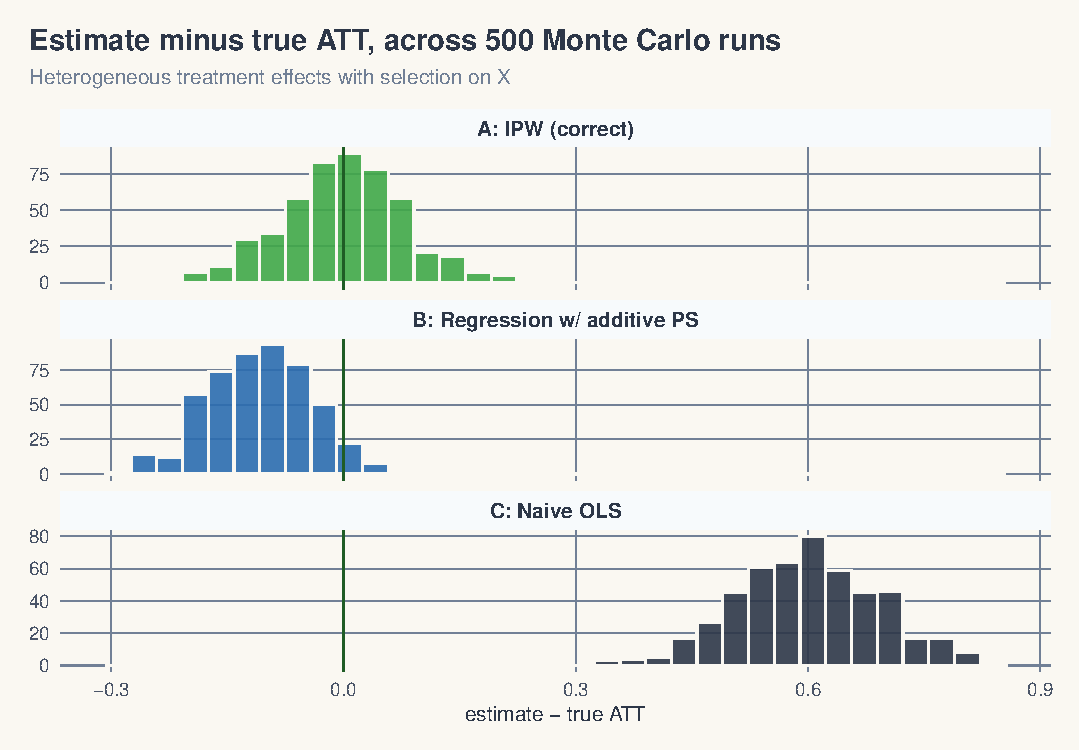
\includegraphics[width=0.86\linewidth,height=0.70\textheight,keepaspectratio]{figures/ipw_comparison.pdf}
\end{center}
\vspace{-0.4em}
\begin{center}
\footnotesize\color{warmgray}\itshape
500 reps. Heterogeneous $\tau(X) = 1 + 0.5\, X_1$.\;
Method A (IPW reweighting): bias $\approx 0$. \;
Method B (regression with $\widehat{p}$): \highlight{bias $\approx -10\%$}.
\end{center}
\end{frame}

%% ---------- L4-F4: codeblock ----------
\begin{frame}[fragile]{The simulation, one screen of R}
\vspace{0.1em}
\begin{lstlisting}[language=R,basicstyle=\ttfamily\scriptsize]
N  <- 1000
X1 <- rnorm(N); X2 <- rnorm(N)
p  <- plogis(0.5*X1 + 0.3*X2 - 0.2)        # true propensity
D  <- rbinom(N, 1, p)
Y0 <- X1 + 0.5*X2 + rnorm(N)
Y1 <- Y0 + (1 + 0.5*X1)                    # heterogeneous tau(X)
Y  <- D*Y1 + (1-D)*Y0

phat <- glm(D ~ X1 + X2, family=binomial)$fitted.values

# Method A: IPW -- reweight controls
w  <- ifelse(D==1, 1, phat/(1-phat))
A  <- mean(Y[D==1]) - weighted.mean(Y[D==0], w[D==0])

# Method B: regression with pscore as a control
B  <- coef(lm(Y ~ D + phat))["D"]          # <-- the trap
\end{lstlisting}
\meta{Full simulation: \texttt{decks/code/IPW-Demo/ipw\_simulation.R}}
\end{frame}

%% ---------- L4-F5: the intuition ----------
\begin{frame}{Weight versus regressor --- different uses of the same scalar}
\vspace{0.4em}
\begin{itemize}
  \item The propensity score is a \highlight{tool}. The same scalar can be used as:
  \begin{itemize}\small
    \item[--] a \textbf{weight} (Method A: reweight controls) --- recovers ATT
    \item[--] a \textbf{regressor} (Method B: add as control) --- imposes homogeneous effects
  \end{itemize}
  \item Same number. Different uses. \textit{Different identifying assumptions.}
  \item Method B's bias is not noise. It is the heterogeneity in $\tau(X)$ that the regression cannot see.
\end{itemize}
\vspace{0.5em}
\begin{block}{The lesson before DR}
\small
``Doubly robust'' is sometimes mis-summarized as ``IPW plus a regression control.'' \\[0.2em]
\highlight{That's wrong.} DR is something else --- it uses the pscore as a weight, AND it uses an outcome model. \\
But it does NOT use the pscore as a regressor.
\end{block}
\end{frame}

%% ---------- L4-F6: name the disease ----------
\begin{frame}{Name the disease: \textit{additive-control-side bias}}
\vspace{0.4em}
Whenever you put a covariate on the right-hand side of an outcome regression \textit{additively} (no $D \times X$ interaction), you force:
\vspace{-0.2em}
\[
\tau \;\;\text{is constant across all values of that covariate.}
\]
\vspace{-0.4em}
\begin{itemize}\small
  \item Method B (Lesson 4): the covariate is $\widehat{p}(X)$ --- a scalar summary of $X$. \\
        Force constant $\tau$ across $\widehat{p}(X)$. Heterogeneity in $\tau(X)$ is invisible.
  \item TWFE-with-controls (Lesson 2): the covariate is $X$ itself. \\
        Force constant $\tau$ across $X$. Heterogeneity in $\tau(X)$ is invisible.
  \item \highlight{Same disease, different costume.} Caetano \& Callaway (2024) name the TWFE version \textit{hidden linearity bias}. It's the same root.
\end{itemize}
\vspace{0.3em}
\begin{center}
\small\color{warmgray}\itshape
DR's escape: use $X$ and $\widehat{p}(X)$ as \textit{weights} and to model the \textit{counterfactual} $\mu_0(X)$ on controls only --- never as additive regressors of $Y$.
\end{center}
\end{frame}

%% =====================================================================
%%                                LESSON 5
%% =====================================================================
\remixsection{5.\ Doubly Robust DiD}

%% ---------- L5-F1: the idea ----------
\begin{frame}{Doubly robust: two chances to be right}
\vspace{0.4em}
\begin{itemize}
  \item OR needs $\widehat{\mu}_0(X)$ correctly specified.
  \item IPW needs $\widehat{p}(X)$ correctly specified.
  \item Neither is foolproof. Each fails if its own model is wrong.
\end{itemize}
\vspace{0.5em}
\begin{block}{The Sant'Anna \& Zhao (2020) move}
\small
Combine them. The \textbf{DR-DiD} estimator is consistent if \textit{either} model is correct --- not necessarily both.
\end{block}
\vspace{0.4em}
\highlight{Two chances to be right.} \;\; That is what ``doubly robust'' means.
\end{frame}

%% ---------- L5-F1b: identification assumptions ----------
\begin{frame}{DR-DiD identification: three assumptions}
\footnotesize
\begin{block}{Assumption 1 (Data)}
Panel or repeated cross-sections with pre- and post-periods; treatment in post-period; covariates $X$ pre-treatment.
\end{block}
\begin{block}{Assumption 2 (Conditional parallel trends)}
\centering
$\mathbb{E}[\Delta Y(0) \mid D{=}1, X] \;=\; \mathbb{E}[\Delta Y(0) \mid D{=}0, X]$
\end{block}
\begin{block}{Assumption 3 (Common support)}
\centering
$0 \;<\; p(X) \;<\; 1$ \;for almost every $X$.
\end{block}
\begin{center}
\itshape\color{warmgray}
DR-DiD + these three $\Rightarrow$ ATT identified if either model is correct. Proof next slide.
\end{center}
\end{frame}

%% ---------- L5-F2: the formula ----------
\begin{frame}{The DR-DiD estimator}
\vspace{0.4em}
\small
\[
\widehat{\delta}_{\text{DR}} \;=\; \mathbb{E}\!\left[\;
\Bigg(\frac{D}{\mathbb{E}[D]} \;-\; \frac{\frac{p(X)(1-D)}{1-p(X)}}{\mathbb{E}\!\big[\frac{p(X)(1-D)}{1-p(X)}\big]}\Bigg)\,\big(\Delta Y \;-\; \mu_0(X)\big)
\;\right]
\]
\vspace{0.3em}
\begin{itemize}\small
  \item $p(X)$: propensity score model
  \item $\mu_0(X)$: outcome model fitted on \textit{controls}: \;\;$\mu_0(X) \;=\; \mathbb{E}[\Delta Y \mid D{=}0, X]$
  \item The IPW weight reweights the comparison. The OR term centers the residual on the imputed counterfactual.
  \item If $p$ is right, the IPW piece does the work. If $\mu_0$ is right, the OR piece does the work. Proof next slide.
\end{itemize}
\end{frame}

%% ---------- L5-F2b: PROOF — double robustness ----------
\begin{frame}{Proof: doubly robust --- \textit{either} model can be wrong}
\footnotesize
Let $w(X)$ denote the weight operator in $\widehat\delta_{\text{DR}} = \mathbb{E}[w(X)(\Delta Y - \mu_0(X))]$.
\vspace{0.4em}

\textbf{Case A: $p(X)$ correct, $\mu_0(X)$ may be wrong.}
\vspace{-0.2em}
\[
\widehat\delta_{\text{DR}} \;=\; \underbrace{\mathbb{E}[w(X)\,\Delta Y]}_{\text{IPW identifies ATT}}
\;-\; \underbrace{\mathbb{E}[w(X)\,\mu_0(X)]}_{=\;0 \text{ in expectation}} \;=\; \text{ATT.}
\]
The OR term vanishes because $\mathbb{E}[w(X) \mid X] = 0$ once $p(X)$ is correct. \highlight{IPW alone identifies the ATT.}
\vspace{0.5em}

\textbf{Case B: $\mu_0(X)$ correct, $p(X)$ may be wrong.}\;\;Under conditional PT, the residual $\Delta Y - \mu_0(X)$ has conditional mean zero given $D{=}0, X$:
\vspace{-0.2em}
\[
\mathbb{E}[\Delta Y - \mu_0(X) \mid D{=}0, X] \;=\; 0,
\]
\vspace{-0.2em}
so the control piece zeroes regardless of weighting. The treated piece $\tfrac{D}{\mathbb{E}[D]}(\Delta Y - \mu_0(X))$ integrates directly to the ATT. \highlight{OR alone identifies the ATT.}
\vspace{0.4em}

\begin{center}
\footnotesize\color{warmgray}\itshape
Either suffices --- not both. \;That is ``two chances to be right.'' \;$\blacksquare$
\end{center}
\end{frame}

%% ---------- L5-F3: not pscore as regressor ----------
\begin{frame}{DR is \textit{not} regression-with-pscore}
\vspace{0.4em}
\begin{itemize}
  \item Look at the formula. \highlight{$\widehat{p}(X)$ appears as a weight, never as a regressor.}
  \item $\mu_0(X)$ models the outcome, but on \textit{controls only} --- to impute the counterfactual trend.
  \item The two pieces are combined by a re-centering and reweighting, NOT by adding $\widehat{p}$ to a regression's right-hand side.
\end{itemize}
\vspace{0.6em}
\begin{center}
\small\color{warmgray}\itshape
The pscore is the tool. \highlight{Using it as a weight is doubly robust.} Using it as a regressor is the trap from Lesson 4.
\end{center}
\end{frame}

%% ---------- L5-F4: efficiency ----------
\begin{frame}{Efficiency and the influence function}
\vspace{0.4em}
\begin{itemize}\small
  \item Under conditional PT + common support, DR-DiD is \highlight{semiparametrically efficient}.
  \item No estimator of the ATT that uses only the same assumptions can have a smaller asymptotic variance.
  \item The asymptotic variance has a closed form via the \textit{influence function} (this is what the \texttt{drdid} package computes for SEs).
\end{itemize}
\vspace{0.5em}
\begin{block}{Practical recipe}
\small
Pick $X$ for confounding (Lesson 1). \;\; Estimate $\widehat{p}(X)$ by logit. \;\; Estimate $\widehat{\mu}_0(X)$ on controls. \;\; Plug into the DR-DiD formula. \;\; Influence-function SEs.
\end{block}
\end{frame}

%% ---------- L5-F5: live code ----------
\begin{frame}[fragile]{DR-DiD, in code}
\vspace{0.2em}
\begin{lstlisting}[language=R]
library(DRDID)

# Panel data: outcome y, treatment indicator d, time t, id, covariates X
result <- drdid(
  yname        = "y",
  tname        = "t",
  idname       = "id",
  dname        = "d",
  xformla      = ~ x1 + x2 + x3,    # covariates for BOTH p(X) and mu_0(X)
  data         = panel_df,
  estMethod    = "imp",             # Sant'Anna & Zhao (2020) DR
  weightsname  = NULL,
  boot         = FALSE,
  inffunc      = TRUE               # influence-function SEs
)
summary(result)
\end{lstlisting}
\vspace{0.1em}
\meta{Same X used for both models. Misspecify one --- the other catches you.}
\end{frame}

%% =====================================================================
%%                                LESSON 6
%%        Caetano & Callaway: hidden linearity bias (same disease as L4)
%% =====================================================================
\remixsection{6.\ Hidden Linearity Bias \\[0.3em] {\normalsize\normalfont Caetano \& Callaway 2024}}

%% ---------- L6-F0: TWFE-with-controls has TWO distinct problems ----------
\begin{frame}{TWFE-with-controls has two distinct problems}
\vspace{0.4em}
The workhorse specification $Y_{it} = \alpha_i + \gamma_t + \tau D_{it} + X_{it}'\beta + \varepsilon_{it}$ is biased for two \textit{separate} reasons:
\vspace{0.5em}
\begin{enumerate}
  \item \highlight{The FE transformation throws away what you wanted to control for.} \\[0.2em]
  First-differencing $X_{it}$ leaves only $\Delta X$. The \textit{level} of $X$ is gone. Time-invariant $Z$ is gone entirely. \;\; (Caetano-Callaway 2024 --- this lesson.)
  \item \highlight{What's left enters additively, forcing constant $\tau$.} \\[0.2em]
  Whatever covariate survives the FE transformation sits on the RHS as an additive regressor with no $D{\times}X$ interaction. Same disease as Method B (Lesson 4).
\end{enumerate}
\vspace{0.5em}
\begin{center}
\small\color{warmgray}\itshape
This lesson covers problem (1). Problem (2) is the L4 callback we'll close on.
\end{center}
\end{frame}

%% ---------- L6-F1: the applied problem ----------
\begin{frame}{An applied problem you've already run}
\vspace{0.5em}
\pullquote{TWFE with time-varying controls is the workhorse DiD specification. Almost every DiD paper runs it.}{Anybody who's seen a job-market paper}
\vspace{0.5em}
\begin{itemize}
  \item Standard recipe: include population, income, demographic shares, region indicators, etc. on the right-hand side. Run TWFE. Done.
  \item \highlight{What if I told you that regression doesn't control for what you think it controls for?}
  \item Caetano \& Callaway (2024, R\&R \textit{REStat}): yes. The fixed-effect transformation quietly drops your $X$ levels and your time-invariant $Z$.
\end{itemize}
\end{frame}

%% ---------- L6-F2: the application — SYG laws ----------
\begin{frame}{An application: stand-your-ground laws (Cheng \& Hoekstra 2013)}
\vspace{0.5em}
\begin{itemize}\small
  \item 50 states, 2000--2010. 20 states adopt stand-your-ground laws. Outcome: log homicide rate.
  \item Treated states differ from controls in \highlight{levels}:
  \begin{itemize}\small
    \item[--] South dummy: std.\ diff. $= 0.81$  (large)
    \item[--] Poverty rate:  std.\ diff. $= 1.06$  (huge)
    \item[--] Median income: std.\ diff. $= -1.08$ (huge)
  \end{itemize}
  \item But the differences in \highlight{changes} of these covariates are small.
\end{itemize}
\vspace{0.6em}
\begin{block}{The headline result}
\small
TWFE with covariates: \;\;$\widehat{\alpha} = +0.067$, \;significant. \\
AIPW with the right covariates: \;$\widehat{\text{ATT}} \approx 0$, insignificant.\\[0.3em]
\highlight{The positive TWFE result is largely artefact of hidden linearity bias.}
\end{block}
\end{frame}

%% ---------- L6-F3: the intuition ----------
\begin{frame}{What TWFE actually controls for, after the FE transformation}
\vspace{0.4em}
You wrote down this model:
\vspace{-0.1em}
\[
Y_{it} \;=\; \alpha_i \;+\; \gamma_t \;+\; \tau D_{it} \;+\; X_{it}'\beta \;+\; Z_i'\delta \;+\; \varepsilon_{it}
\]
\vspace{0.1em}
First-difference (or within-transform) to kill $\alpha_i$:
\vspace{-0.2em}
\[
\Delta Y_{it} \;=\; \widetilde{\gamma}_t \;+\; \tau\, \Delta D_{it} \;+\; \Delta X_{it}'\beta \;+\; \Delta \varepsilon_{it}
\]
\vspace{0.1em}
\begin{itemize}\small
  \item $\alpha_i$ vanishes (good).
  \item $Z_i$ vanishes too (time-invariant). \highlight{Region: gone.}
  \item $X_{it}$ becomes $\Delta X_{it}$. \highlight{Population level: gone. Only population growth remains.}
  \item Your ``controls'' are now \textit{changes} in $X$, not levels.
\end{itemize}
\end{frame}

%% ---------- L6-F4: what the correct model is ----------
\begin{frame}{What you should be controlling for}
\vspace{0.5em}
The correct first-differenced model for $\Delta Y(0)$ (Caetano-Callaway Eq.\ 4):
\vspace{-0.2em}
\[
\Delta Y_{it}(0) \;=\; \widetilde{\gamma}_t \;+\; \underbrace{Z_i'\widetilde{\delta}_t}_{\text{time-inv}}
                                         \;+\; \underbrace{\Delta X_{it}'\beta_t}_{\text{changes}}
                                         \;+\; \underbrace{X_{i,t-1}'\widetilde{\beta}_t}_{\text{level}}
                                         \;+\; \Delta\varepsilon_{it}
\]
\vspace{0.1em}
\begin{itemize}\small
  \item \textbf{Time-invariant} $Z$ (region) belongs on the right --- because trends differ by region.
  \item \textbf{Pre-period level} $X_{i,t-1}$ belongs on the right --- because the level of population predicts the trend in homicides.
  \item TWFE drops both. \highlight{Hidden linearity bias.}
\end{itemize}
\end{frame}

%% ---------- L6-F5: the callback to Lesson 4 ----------
\begin{frame}{The L4 callback: problem (2) is the additive-RHS disease}
\vspace{0.3em}
We've covered problem (1) above --- the FE transformation throws away levels. \\
Problem (2) is the L4 disease, present in TWFE-with-controls too.
\vspace{0.4em}
\begin{center}
\renewcommand{\arraystretch}{1.4}
\footnotesize
\begin{tabular}{@{}lll@{}}
\toprule
\textbf{Estimator} & \textbf{What goes on RHS additively} & \textbf{What gets forced constant} \\
\midrule
\rowcolor{remixgreenlight}
Method B (L4)             & $\widehat{p}(X)$ as control          & $\tau$ across $\widehat{p}(X)$ \\
\rowcolor{remixgreenlight}
TWFE-with-controls (L2, L6) & $\Delta X$ as control              & $\tau$ across $\Delta X$       \\
\rowcolor{remixgreenlight}
General formulation       & $W = f(X)$ as additive RHS regressor & $\tau$ across $W$              \\
\bottomrule
\end{tabular}
\end{center}
\vspace{0.3em}
\begin{itemize}\small
  \item Problem (1) is C\&C's contribution: \textit{what} you control for is wrong.
  \item Problem (2) is the L4 disease: \textit{how} you control for it is wrong.
  \item TWFE-with-controls catches both. DR escapes both --- using $X$ and $\widehat{p}(X)$ as \highlight{weights}, not as additive regressors.
\end{itemize}
\end{frame}

%% ---------- L6-F6: the fix — AIPW ----------
\begin{frame}{The fix: AIPW with $(X_{t-1},\, Z)$}
\vspace{0.5em}
Caetano-Callaway's recommended estimator:
\vspace{-0.1em}
\[
\widehat{\text{ATT}} \;=\; \widehat{\mathbb{E}}_{D=1}\!\big[\Delta Y \;-\; \widehat{m}_0(X_{t-1}, Z)\big]
\]
\vspace{0.1em}
\begin{itemize}\small
  \item $\widehat{m}_0(X_{t-1}, Z)$: outcome regression of $\Delta Y$ on \textit{pre-period level} of $X$ and \textit{time-invariant} $Z$ --- fit on \textbf{controls only}.
  \item Combine with IPW on a generalized propensity score (also using $X_{t-1}, Z$) for full doubly-robust safety.
  \item R packages: \texttt{pte}, \texttt{twfeweights}.
  \item This is just DR-DiD (L5) with the \textit{right} conditioning set: levels of time-varying $X$ + time-invariant $Z$.
\end{itemize}
\end{frame}

%% ---------- L6-F7: SYG numbers ----------
\begin{frame}{Stand-your-ground revisited --- the numbers}
\vspace{0.5em}
\begin{center}
\renewcommand{\arraystretch}{1.4}
\footnotesize
\begin{tabular}{@{}lcc@{}}
\toprule
\textbf{Specification}                                & \textbf{$\widehat{\text{ATT}}$} & \textbf{SE} \\
\midrule
TWFE with $\Delta X$ (the standard recipe)            & $+0.067$               & 0.026       \\
Reg.\ adj.\ with $\Delta X + Z$                        & $+0.106$               & 0.058       \\
\rowcolor{remixgreenlight}
Reg.\ adj.\ with $X_{t-1} + Z$ \;(\textit{Caetano-Callaway preferred}) & $+0.019$ & 0.043 \\
Reg.\ adj.\ with $\Delta X + X_{t-1} + Z$              & $+0.078$               & 0.180       \\
\bottomrule
\end{tabular}
\end{center}
\vspace{0.6em}
\begin{itemize}\small
  \item The TWFE positive effect ($+6.7\%$) shrinks to near-zero ($+1.9\%$) when you control for \textit{levels} of $X$ and $Z$.
  \item The bias was hidden in plain sight --- the regression compiled fine. It just wasn't controlling for what we thought.
\end{itemize}
\end{frame}

%% =====================================================================
%%                                LESSON 7
%% =====================================================================
\remixsection{7.\ Compositional Change}

%% ---------- L7-F1: a different X-moves problem ----------
\begin{frame}{Two flavors of ``$X$ moves''}
\vspace{0.4em}
\begin{center}
\renewcommand{\arraystretch}{1.4}
\footnotesize
\begin{tabular}{@{}lll@{}}
\toprule
\textbf{Flavor} & \textbf{What's moving} & \textbf{Estimator} \\
\midrule
\textbf{Lesson 6} & Same units, $X_{it}$ moves over time & Caetano-Callaway AIPW \\[0.1em]
\textbf{Lesson 7} & New units each period, $X$ distribution moves & Hong / Sant'Anna-Xu \\
\bottomrule
\end{tabular}
\end{center}
\vspace{0.6em}
\begin{itemize}\small
  \item Both break unconditional PT \textit{in finite samples} even when it holds in the population.
  \item L6 (panel): the FE transformation loses the $X$ level. \;\; L7 (repeated cross-sections): the sample composition shifts.
  \item Different fixes. Same family of concerns: \highlight{$X$ is moving, and your estimator pretends it isn't.}
\end{itemize}
\end{frame}

%% ---------- L7-F2: Hong Napster ----------
\begin{frame}{Hong (2013): Napster, internet users, and music expenditure}
\vspace{0.5em}
\begin{itemize}
  \item Repeated cross-sections, 1996 and 2002.
  \item In 1996, internet users were a small, atypical slice --- mostly young, urban, technical.
  \item By 2002, internet users looked much more like the general population.
  \item Compare ``internet users'' to ``non-users,'' 1996 vs.\ 2002. \\ \highlight{Did Napster reduce music spending --- or did the composition of internet users change?}
  \item Hong's answer: the naive DiD confounds the two. The compositional shift accounts for much of the apparent ``Napster effect.''
\end{itemize}
\vspace{0.4em}
\meta{Hong (2013) JEEA. Figures in \texttt{CI-2/lecture\_includes/hong\_napster.png}.}
\end{frame}

%% ---------- L7-F3: bridge — what's left for SX ----------
\begin{frame}{So why do we need Sant'Anna \& Xu given Hong showed it?}
\vspace{0.4em}
Hong (2013) gave us the intuition --- and a single empirical example. To use this in your own work you need three things Hong didn't formalize:
\vspace{0.4em}
\begin{enumerate}\small
  \item \textbf{A target estimand.} What \textit{is} ``the'' ATT under compositional shift? Is it the average over the post-period sample (your data) or the pre-period sample? These are different parameters.
  \item \textbf{A test.} Hong showed his data had the problem. How do \textit{you} know yours does, without the benefit of a second empirical paper?
  \item \textbf{A correction.} If your test rejects, what estimator should you report? Hong didn't give you one --- he flagged the problem.
\end{enumerate}
\end{frame}

%% ---------- L7-F3b: the one-line punchline ----------
\begin{frame}[plain]
\begin{tikzpicture}[remember picture,overlay]
\fill[cream] (current page.south west) rectangle (current page.north east);
\node[anchor=center, text width=0.82\paperwidth, align=center, text=charcoal] at (current page.center) {%
  \fontsize{22pt}{30pt}\selectfont
  The story stays {\color{accent}\bfseries Hong's.}\\[0.4em]
  The toolkit is {\color{accent}\bfseries new.}
};
\end{tikzpicture}
\end{frame}

%% ---------- L7-F4a: SX — the estimand ----------
\begin{frame}{Sant'Anna \& Xu: first, fix an estimand}
\vspace{0.5em}
\pullquote{What \textit{is} ``the'' ATT when the sample composition is moving?}{Anyone trying to use Hong in their own paper}
\vspace{0.7em}
\begin{block}{The SX target}
The population ATT averaged over a \highlight{fixed reference $X$-distribution} --- typically the pre-period.
\end{block}
\vspace{0.4em}
\begin{itemize}
  \item The naive DiD targets a \textit{moving} mixture --- a weighted average of period-specific ATTs, weighted by whatever happened to be in each period's sample.
  \item Pick a reference. Now you know what number you're trying to estimate.
\end{itemize}
\end{frame}

%% ---------- L7-F4b: SX — the test ----------
\begin{frame}{Second, test for compositional shift}
\vspace{0.6em}
\begin{block}{Hausman-style test}
\small
Compute the naive DiD. Compute the DiD on the sample \textit{reweighted to the reference $X$-distribution}. Compare.
\end{block}
\vspace{0.6em}
\begin{itemize}
  \item Under the null (no compositional shift), the two estimates agree.
  \item Under the alternative, they diverge --- and the gap is informative about how much your point estimate is doing compositional vs.\ behavioral work.
  \item Standard $\chi^2$ inference.
\end{itemize}
\vspace{0.3em}
\begin{center}
\small\color{warmgray}\itshape
This is the move Hong didn't have. He showed his data had the problem. The Hausman test lets \textit{you} check yours.
\end{center}
\end{frame}

%% ---------- L7-F4c: SX — the estimator ----------
\begin{frame}{Third, reweight and estimate}
\vspace{0.6em}
\begin{block}{The SX estimator}
\small
Reweight units in each period so the within-period $X$-distribution matches the chosen reference. Then compute DiD on the reweighted sample.
\end{block}
\vspace{0.6em}
\begin{itemize}
  \item Mechanically: IPW-style reweighting, with weights derived from $f_{\text{ref}}(X) / f_t(X)$ at each period.
  \item \highlight{Doubly robust} version available --- combine the IPW reweighting with an outcome model (callback to Lesson 5).
  \item Software: implementable from the IPW machinery you already know.
\end{itemize}
\end{frame}

%% ---------- L7-F5: when this matters ----------
\begin{frame}{When compositional change matters in practice}
\vspace{0.5em}
\begin{itemize}
  \item \textbf{Survey data over long horizons.} CPS, NLSY, ACS --- sample composition drifts as response rates, demographics, frame definitions change.
  \item \textbf{Administrative outcomes with selective coverage.} Who enters the data may itself respond to policy (Medicaid take-up, charter-school enrollment).
  \item \textbf{New technology adoption.} Hong's Napster, again. The adopter pool changes over time --- almost by definition.
  \item \textbf{Long pre-periods in event studies.} The further back you go, the more likely the population you're comparing has shifted.
\end{itemize}
\vspace{0.3em}
\begin{center}
\small\color{warmgray}\itshape
First defense: check whether $X$ distribution moved across time. Then run the Hausman test. Then report both estimates.
\end{center}
\end{frame}

%% =====================================================================
%%                                ACT III
%% =====================================================================

%% ---------- Lab: LaLonde with covariates ----------
\begin{frame}{Lab: LaLonde under selection (\textit{the four estimators, one truth})}
\vspace{0.3em}
\begin{itemize}\small
  \item \textbf{The benchmark.} The experimental NSW sample identifies the ATT by random assignment: \;\highlight{$\widehat{\text{ATT}}^{\text{RCT}} \approx \$1{,}700$ (1978 dollars)}. Compute it first.
  \item \textbf{The non-experimental panel.} NSW treated $+$ a random CPS sample as the control. Selection bias is large and \textit{negative} --- naive DiD gives the wrong sign.
  \item \textbf{Run all four estimators}, get an ATT, compare to \$1{,}700:
  \begin{itemize}\footnotesize
    \item[--] \textbf{TWFE-with-X} (interact Post $\times\;X$ --- without the interaction, FE sweeps them out)
    \item[--] \textbf{OR} (Heckman--Ichimura--Todd 1997)
    \item[--] \textbf{IPW} (Abadie 2005)
    \item[--] \textbf{DR-DiD} (Sant'Anna--Zhao 2020): \texttt{drdid} with the \texttt{all} option
  \end{itemize}
  \item \textbf{Then answer:} which estimators move the ATT in the right direction? Which get closest? When does DR \textit{not} dominate? What does the propensity-score overlap plot show?
\end{itemize}
\vspace{0.3em}
\meta{Walkthrough: \texttt{zurich/labs/Lalonde-Covariates/README.md}. \;Data: \texttt{lalonde\_exp\_panel.dta} \& \texttt{lalonde\_nonexp\_panel.dta} on Mixtape-Sessions GitHub.}
\end{frame}

%% ---------- Recap ----------
\begin{frame}{What we've done this afternoon}
\vspace{0.3em}
\begin{enumerate}\small
  \item Conditional PT --- the new identifying assumption
  \item Outcome regression: model the trend, impute the counterfactual
  \item IPW: reweight controls to look like the treated
  \item The trap: ``controlling for the pscore'' imposes constant $\tau$ across $\widehat{p}(X)$
  \item Doubly robust: pscore as a \textit{weight} (not regressor) + outcome model
  \item Hidden linearity bias (Caetano-Callaway): \textit{same disease}, costume = TWFE-with-controls
  \item Compositional change (Hong; Sant'Anna-Xu): when the \textit{units} shift, not $X$
\end{enumerate}
\vspace{0.5em}
\begin{center}
\small\color{warmgray}\itshape
The unifying lesson: covariates on the additive RHS of an outcome regression impose constraints on $\tau$. \\
DR's escape is to use them as \highlight{weights}, not regressors.
\end{center}
\end{frame}

%% ---------- Tomorrow preview ----------
\begin{frame}{Tomorrow}
\vspace{0.4em}
\begin{itemize}
  \item \textbf{Day 3:} when even covariates can't save you. Synthetic control, the frontier methods.
  \item Plus: when treatment timing differs across units --- the staggered-adoption mess (Goodman-Bacon, Callaway-Sant'Anna, Sun-Abraham, BJS, dCdH).
\end{itemize}
\end{frame}

%% ---------- Closing one-sentence linger ----------
\begin{frame}[plain]
\begin{tikzpicture}[remember picture,overlay]
\fill[cream] (current page.south west) rectangle (current page.north east);
\node[anchor=center, text width=0.84\paperwidth, align=center, text=charcoal] at (current page.center) {%
  \fontsize{18pt}{26pt}\selectfont
  Use the pscore as a {\color{accent}\bfseries weight,}\\[0.3em]
  not as a {\color{accent}\bfseries regressor.}\\[0.6em]
  That is the difference between {\color{accent}\bfseries doubly robust}\\[0.2em]
  and {\color{accent}\bfseries doubly biased.}
};
\draw[accent, line width=1pt] ([yshift=1.4cm,xshift=0.25\paperwidth]current page.south west) -- ([yshift=1.4cm,xshift=-0.25\paperwidth]current page.south east);
\end{tikzpicture}
\end{frame}

\end{document}
